\documentclass[border=4pt]{standalone}
\usepackage{amsmath,amssymb}
\usepackage{tikz}
\usetikzlibrary{arrows.meta,decorations.pathreplacing}
\begin{document}
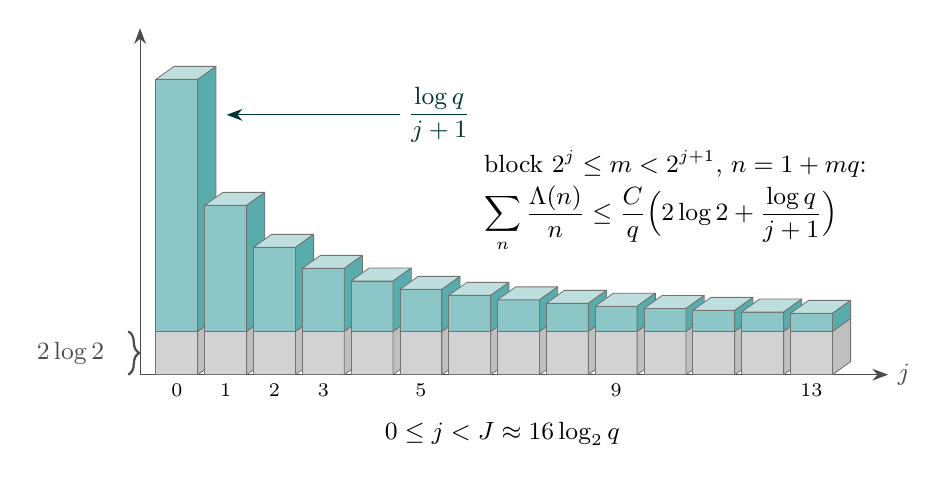
\begin{tikzpicture}[line join=round,>={Stealth[length=2mm]}]
  \draw[->,gray!60!black] (-0.2,0)--(9.3,0) node[right,font=\small]{$j$};
  \draw[->,gray!60!black] (-0.2,0)--(-0.2,4.4);
  \filldraw[fill=gray!35,draw=black!55,line width=0.3pt] (0.000,0.000)--(0.533,0.000)--(0.533,0.550)--(0.000,0.550)--cycle;
\filldraw[fill=gray!20,draw=black!55,line width=0.3pt] (0.000,0.550)--(0.533,0.550)--(0.764,0.715)--(0.231,0.715)--cycle;
\filldraw[fill=gray!50,draw=black!55,line width=0.3pt] (0.533,0.000)--(0.764,0.165)--(0.764,0.715)--(0.533,0.550)--cycle;
\filldraw[fill=teal!45,draw=black!55,line width=0.3pt] (0.000,0.550)--(0.533,0.550)--(0.533,3.750)--(0.000,3.750)--cycle;
\filldraw[fill=teal!25,draw=black!55,line width=0.3pt] (0.000,3.750)--(0.533,3.750)--(0.764,3.915)--(0.231,3.915)--cycle;
\filldraw[fill=teal!65,draw=black!55,line width=0.3pt] (0.533,0.550)--(0.764,0.715)--(0.764,3.915)--(0.533,3.750)--cycle;
\node[font=\scriptsize,below] at (0.267,0) {$0$};
\filldraw[fill=gray!35,draw=black!55,line width=0.3pt] (0.620,0.000)--(1.153,0.000)--(1.153,0.550)--(0.620,0.550)--cycle;
\filldraw[fill=gray!20,draw=black!55,line width=0.3pt] (0.620,0.550)--(1.153,0.550)--(1.384,0.715)--(0.851,0.715)--cycle;
\filldraw[fill=gray!50,draw=black!55,line width=0.3pt] (1.153,0.000)--(1.384,0.165)--(1.384,0.715)--(1.153,0.550)--cycle;
\filldraw[fill=teal!45,draw=black!55,line width=0.3pt] (0.620,0.550)--(1.153,0.550)--(1.153,2.150)--(0.620,2.150)--cycle;
\filldraw[fill=teal!25,draw=black!55,line width=0.3pt] (0.620,2.150)--(1.153,2.150)--(1.384,2.315)--(0.851,2.315)--cycle;
\filldraw[fill=teal!65,draw=black!55,line width=0.3pt] (1.153,0.550)--(1.384,0.715)--(1.384,2.315)--(1.153,2.150)--cycle;
\node[font=\scriptsize,below] at (0.887,0) {$1$};
\filldraw[fill=gray!35,draw=black!55,line width=0.3pt] (1.240,0.000)--(1.773,0.000)--(1.773,0.550)--(1.240,0.550)--cycle;
\filldraw[fill=gray!20,draw=black!55,line width=0.3pt] (1.240,0.550)--(1.773,0.550)--(2.004,0.715)--(1.471,0.715)--cycle;
\filldraw[fill=gray!50,draw=black!55,line width=0.3pt] (1.773,0.000)--(2.004,0.165)--(2.004,0.715)--(1.773,0.550)--cycle;
\filldraw[fill=teal!45,draw=black!55,line width=0.3pt] (1.240,0.550)--(1.773,0.550)--(1.773,1.617)--(1.240,1.617)--cycle;
\filldraw[fill=teal!25,draw=black!55,line width=0.3pt] (1.240,1.617)--(1.773,1.617)--(2.004,1.782)--(1.471,1.782)--cycle;
\filldraw[fill=teal!65,draw=black!55,line width=0.3pt] (1.773,0.550)--(2.004,0.715)--(2.004,1.782)--(1.773,1.617)--cycle;
\node[font=\scriptsize,below] at (1.507,0) {$2$};
\filldraw[fill=gray!35,draw=black!55,line width=0.3pt] (1.860,0.000)--(2.393,0.000)--(2.393,0.550)--(1.860,0.550)--cycle;
\filldraw[fill=gray!20,draw=black!55,line width=0.3pt] (1.860,0.550)--(2.393,0.550)--(2.624,0.715)--(2.091,0.715)--cycle;
\filldraw[fill=gray!50,draw=black!55,line width=0.3pt] (2.393,0.000)--(2.624,0.165)--(2.624,0.715)--(2.393,0.550)--cycle;
\filldraw[fill=teal!45,draw=black!55,line width=0.3pt] (1.860,0.550)--(2.393,0.550)--(2.393,1.350)--(1.860,1.350)--cycle;
\filldraw[fill=teal!25,draw=black!55,line width=0.3pt] (1.860,1.350)--(2.393,1.350)--(2.624,1.515)--(2.091,1.515)--cycle;
\filldraw[fill=teal!65,draw=black!55,line width=0.3pt] (2.393,0.550)--(2.624,0.715)--(2.624,1.515)--(2.393,1.350)--cycle;
\node[font=\scriptsize,below] at (2.127,0) {$3$};
\filldraw[fill=gray!35,draw=black!55,line width=0.3pt] (2.480,0.000)--(3.013,0.000)--(3.013,0.550)--(2.480,0.550)--cycle;
\filldraw[fill=gray!20,draw=black!55,line width=0.3pt] (2.480,0.550)--(3.013,0.550)--(3.244,0.715)--(2.711,0.715)--cycle;
\filldraw[fill=gray!50,draw=black!55,line width=0.3pt] (3.013,0.000)--(3.244,0.165)--(3.244,0.715)--(3.013,0.550)--cycle;
\filldraw[fill=teal!45,draw=black!55,line width=0.3pt] (2.480,0.550)--(3.013,0.550)--(3.013,1.190)--(2.480,1.190)--cycle;
\filldraw[fill=teal!25,draw=black!55,line width=0.3pt] (2.480,1.190)--(3.013,1.190)--(3.244,1.355)--(2.711,1.355)--cycle;
\filldraw[fill=teal!65,draw=black!55,line width=0.3pt] (3.013,0.550)--(3.244,0.715)--(3.244,1.355)--(3.013,1.190)--cycle;
\filldraw[fill=gray!35,draw=black!55,line width=0.3pt] (3.100,0.000)--(3.633,0.000)--(3.633,0.550)--(3.100,0.550)--cycle;
\filldraw[fill=gray!20,draw=black!55,line width=0.3pt] (3.100,0.550)--(3.633,0.550)--(3.864,0.715)--(3.331,0.715)--cycle;
\filldraw[fill=gray!50,draw=black!55,line width=0.3pt] (3.633,0.000)--(3.864,0.165)--(3.864,0.715)--(3.633,0.550)--cycle;
\filldraw[fill=teal!45,draw=black!55,line width=0.3pt] (3.100,0.550)--(3.633,0.550)--(3.633,1.083)--(3.100,1.083)--cycle;
\filldraw[fill=teal!25,draw=black!55,line width=0.3pt] (3.100,1.083)--(3.633,1.083)--(3.864,1.248)--(3.331,1.248)--cycle;
\filldraw[fill=teal!65,draw=black!55,line width=0.3pt] (3.633,0.550)--(3.864,0.715)--(3.864,1.248)--(3.633,1.083)--cycle;
\node[font=\scriptsize,below] at (3.367,0) {$5$};
\filldraw[fill=gray!35,draw=black!55,line width=0.3pt] (3.720,0.000)--(4.253,0.000)--(4.253,0.550)--(3.720,0.550)--cycle;
\filldraw[fill=gray!20,draw=black!55,line width=0.3pt] (3.720,0.550)--(4.253,0.550)--(4.484,0.715)--(3.951,0.715)--cycle;
\filldraw[fill=gray!50,draw=black!55,line width=0.3pt] (4.253,0.000)--(4.484,0.165)--(4.484,0.715)--(4.253,0.550)--cycle;
\filldraw[fill=teal!45,draw=black!55,line width=0.3pt] (3.720,0.550)--(4.253,0.550)--(4.253,1.007)--(3.720,1.007)--cycle;
\filldraw[fill=teal!25,draw=black!55,line width=0.3pt] (3.720,1.007)--(4.253,1.007)--(4.484,1.172)--(3.951,1.172)--cycle;
\filldraw[fill=teal!65,draw=black!55,line width=0.3pt] (4.253,0.550)--(4.484,0.715)--(4.484,1.172)--(4.253,1.007)--cycle;
\filldraw[fill=gray!35,draw=black!55,line width=0.3pt] (4.340,0.000)--(4.873,0.000)--(4.873,0.550)--(4.340,0.550)--cycle;
\filldraw[fill=gray!20,draw=black!55,line width=0.3pt] (4.340,0.550)--(4.873,0.550)--(5.104,0.715)--(4.571,0.715)--cycle;
\filldraw[fill=gray!50,draw=black!55,line width=0.3pt] (4.873,0.000)--(5.104,0.165)--(5.104,0.715)--(4.873,0.550)--cycle;
\filldraw[fill=teal!45,draw=black!55,line width=0.3pt] (4.340,0.550)--(4.873,0.550)--(4.873,0.950)--(4.340,0.950)--cycle;
\filldraw[fill=teal!25,draw=black!55,line width=0.3pt] (4.340,0.950)--(4.873,0.950)--(5.104,1.115)--(4.571,1.115)--cycle;
\filldraw[fill=teal!65,draw=black!55,line width=0.3pt] (4.873,0.550)--(5.104,0.715)--(5.104,1.115)--(4.873,0.950)--cycle;
\filldraw[fill=gray!35,draw=black!55,line width=0.3pt] (4.960,0.000)--(5.493,0.000)--(5.493,0.550)--(4.960,0.550)--cycle;
\filldraw[fill=gray!20,draw=black!55,line width=0.3pt] (4.960,0.550)--(5.493,0.550)--(5.724,0.715)--(5.191,0.715)--cycle;
\filldraw[fill=gray!50,draw=black!55,line width=0.3pt] (5.493,0.000)--(5.724,0.165)--(5.724,0.715)--(5.493,0.550)--cycle;
\filldraw[fill=teal!45,draw=black!55,line width=0.3pt] (4.960,0.550)--(5.493,0.550)--(5.493,0.906)--(4.960,0.906)--cycle;
\filldraw[fill=teal!25,draw=black!55,line width=0.3pt] (4.960,0.906)--(5.493,0.906)--(5.724,1.071)--(5.191,1.071)--cycle;
\filldraw[fill=teal!65,draw=black!55,line width=0.3pt] (5.493,0.550)--(5.724,0.715)--(5.724,1.071)--(5.493,0.906)--cycle;
\filldraw[fill=gray!35,draw=black!55,line width=0.3pt] (5.580,0.000)--(6.113,0.000)--(6.113,0.550)--(5.580,0.550)--cycle;
\filldraw[fill=gray!20,draw=black!55,line width=0.3pt] (5.580,0.550)--(6.113,0.550)--(6.344,0.715)--(5.811,0.715)--cycle;
\filldraw[fill=gray!50,draw=black!55,line width=0.3pt] (6.113,0.000)--(6.344,0.165)--(6.344,0.715)--(6.113,0.550)--cycle;
\filldraw[fill=teal!45,draw=black!55,line width=0.3pt] (5.580,0.550)--(6.113,0.550)--(6.113,0.870)--(5.580,0.870)--cycle;
\filldraw[fill=teal!25,draw=black!55,line width=0.3pt] (5.580,0.870)--(6.113,0.870)--(6.344,1.035)--(5.811,1.035)--cycle;
\filldraw[fill=teal!65,draw=black!55,line width=0.3pt] (6.113,0.550)--(6.344,0.715)--(6.344,1.035)--(6.113,0.870)--cycle;
\node[font=\scriptsize,below] at (5.847,0) {$9$};
\filldraw[fill=gray!35,draw=black!55,line width=0.3pt] (6.200,0.000)--(6.733,0.000)--(6.733,0.550)--(6.200,0.550)--cycle;
\filldraw[fill=gray!20,draw=black!55,line width=0.3pt] (6.200,0.550)--(6.733,0.550)--(6.964,0.715)--(6.431,0.715)--cycle;
\filldraw[fill=gray!50,draw=black!55,line width=0.3pt] (6.733,0.000)--(6.964,0.165)--(6.964,0.715)--(6.733,0.550)--cycle;
\filldraw[fill=teal!45,draw=black!55,line width=0.3pt] (6.200,0.550)--(6.733,0.550)--(6.733,0.841)--(6.200,0.841)--cycle;
\filldraw[fill=teal!25,draw=black!55,line width=0.3pt] (6.200,0.841)--(6.733,0.841)--(6.964,1.006)--(6.431,1.006)--cycle;
\filldraw[fill=teal!65,draw=black!55,line width=0.3pt] (6.733,0.550)--(6.964,0.715)--(6.964,1.006)--(6.733,0.841)--cycle;
\filldraw[fill=gray!35,draw=black!55,line width=0.3pt] (6.820,0.000)--(7.353,0.000)--(7.353,0.550)--(6.820,0.550)--cycle;
\filldraw[fill=gray!20,draw=black!55,line width=0.3pt] (6.820,0.550)--(7.353,0.550)--(7.584,0.715)--(7.051,0.715)--cycle;
\filldraw[fill=gray!50,draw=black!55,line width=0.3pt] (7.353,0.000)--(7.584,0.165)--(7.584,0.715)--(7.353,0.550)--cycle;
\filldraw[fill=teal!45,draw=black!55,line width=0.3pt] (6.820,0.550)--(7.353,0.550)--(7.353,0.817)--(6.820,0.817)--cycle;
\filldraw[fill=teal!25,draw=black!55,line width=0.3pt] (6.820,0.817)--(7.353,0.817)--(7.584,0.982)--(7.051,0.982)--cycle;
\filldraw[fill=teal!65,draw=black!55,line width=0.3pt] (7.353,0.550)--(7.584,0.715)--(7.584,0.982)--(7.353,0.817)--cycle;
\filldraw[fill=gray!35,draw=black!55,line width=0.3pt] (7.440,0.000)--(7.973,0.000)--(7.973,0.550)--(7.440,0.550)--cycle;
\filldraw[fill=gray!20,draw=black!55,line width=0.3pt] (7.440,0.550)--(7.973,0.550)--(8.204,0.715)--(7.671,0.715)--cycle;
\filldraw[fill=gray!50,draw=black!55,line width=0.3pt] (7.973,0.000)--(8.204,0.165)--(8.204,0.715)--(7.973,0.550)--cycle;
\filldraw[fill=teal!45,draw=black!55,line width=0.3pt] (7.440,0.550)--(7.973,0.550)--(7.973,0.796)--(7.440,0.796)--cycle;
\filldraw[fill=teal!25,draw=black!55,line width=0.3pt] (7.440,0.796)--(7.973,0.796)--(8.204,0.961)--(7.671,0.961)--cycle;
\filldraw[fill=teal!65,draw=black!55,line width=0.3pt] (7.973,0.550)--(8.204,0.715)--(8.204,0.961)--(7.973,0.796)--cycle;
\filldraw[fill=gray!35,draw=black!55,line width=0.3pt] (8.060,0.000)--(8.593,0.000)--(8.593,0.550)--(8.060,0.550)--cycle;
\filldraw[fill=gray!20,draw=black!55,line width=0.3pt] (8.060,0.550)--(8.593,0.550)--(8.824,0.715)--(8.291,0.715)--cycle;
\filldraw[fill=gray!50,draw=black!55,line width=0.3pt] (8.593,0.000)--(8.824,0.165)--(8.824,0.715)--(8.593,0.550)--cycle;
\filldraw[fill=teal!45,draw=black!55,line width=0.3pt] (8.060,0.550)--(8.593,0.550)--(8.593,0.779)--(8.060,0.779)--cycle;
\filldraw[fill=teal!25,draw=black!55,line width=0.3pt] (8.060,0.779)--(8.593,0.779)--(8.824,0.944)--(8.291,0.944)--cycle;
\filldraw[fill=teal!65,draw=black!55,line width=0.3pt] (8.593,0.550)--(8.824,0.715)--(8.824,0.944)--(8.593,0.779)--cycle;
\node[font=\scriptsize,below] at (8.327,0) {$13$};

  \draw[decorate,decoration={brace,amplitude=4pt,mirror},thick,gray!60!black] (-0.35,0)--(-0.35,0.55)
     node[midway,left=5pt,font=\small,align=right] {$2\log 2$};
  \node[font=\small,align=left,teal!40!black] at (3.6,3.3) {$\dfrac{\log q}{j+1}$};
  \draw[->,teal!40!black] (3.1,3.3)--(0.9,3.3);
  \node[font=\small,align=left] at (6.6,2.2) {block $2^j\le m<2^{j+1}$, $n=1+mq$:\\[2pt]
       $\displaystyle\sum_{n}\frac{\Lambda(n)}n\le\frac{C}{q}\Bigl(2\log2+\frac{\log q}{j+1}\Bigr)$};
  \node[font=\small] at (4.4,-0.75) {$0\le j<J\approx 16\log_2 q$};
\end{tikzpicture}
\end{document}
